\chapter{DEPLOYMENT}
\section{Folder Structure}
\begin{figure}[H]
    \centering
    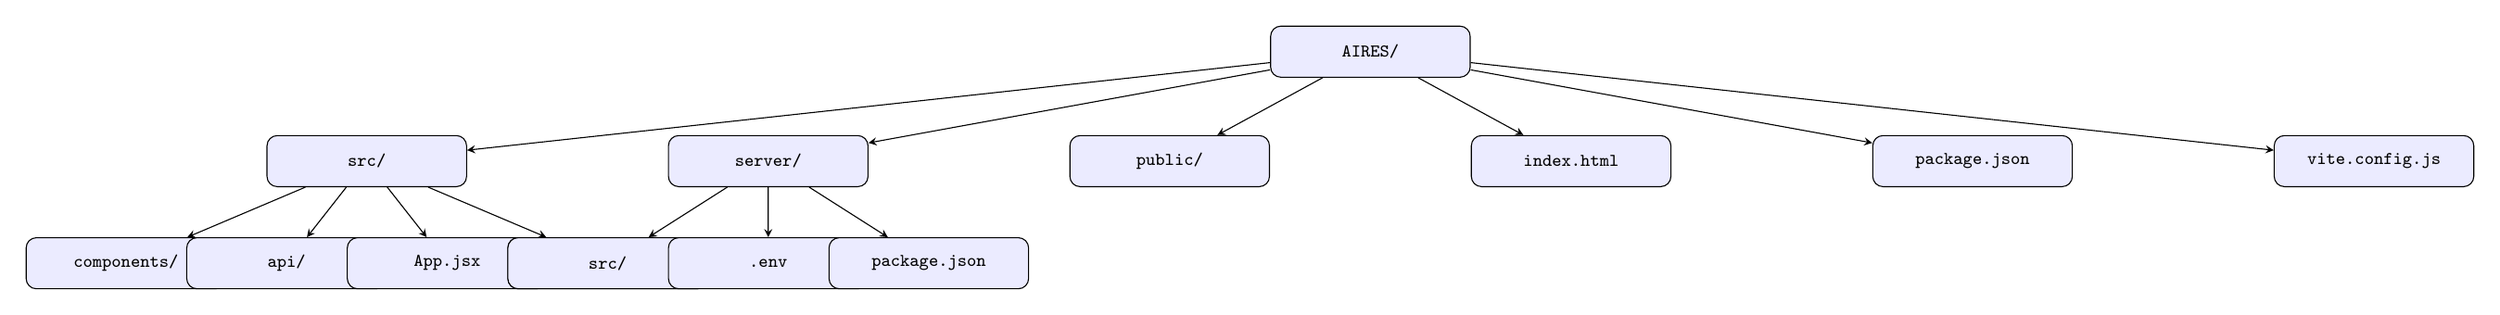
\begin{tikzpicture}[
        font=\ttfamily\small,
        edge from parent/.style={draw, ->, >=stealth},
        level 1/.style={sibling distance=5.5cm, level distance=1.5cm},
        level 2/.style={sibling distance=2.2cm, level distance=1.4cm},
        level 3/.style={sibling distance=1.5cm, level distance=1.3cm},
        every node/.style={rectangle, draw, rounded corners, fill=blue!8, align=center, minimum height=0.7cm, text width=2.5cm, font=\scriptsize\ttfamily}
    ]
        \node {AIRES/}
            child { node {src/}
                child { node {components/} }
                child { node {api/} }
                child { node {App.jsx} }
                child { node {index.css} }
            }
            child { node {server/}
                child { node {src/} }
                child { node {.env} }
                child { node {package.json} }
            }
            child { node {public/} }
            child { node {index.html} }
            child { node {package.json} }
            child { node {vite.config.js} };
    \end{tikzpicture}
    \caption{AIRES Project Folder Structure}
    \label{fig:folder_structure}
\end{figure}

\section{Deployment Process}
The AIRES application is structured as a monorepo containing two separately deployable sub-applications: the React frontend and the Node.js/Express backend. The deployment workflow for each layer is described below.\\\\
\textbf{Frontend Deployment (Vite + React):}
\begin{enumerate}
    \item Navigate to the project root directory.
    \item Install all Node.js dependencies: \texttt{npm install}
    \item Create a production build using Vite: \texttt{npm run build}
    \item The \texttt{dist/} folder contains the compiled static assets.
    \item Deploy the \texttt{dist/} folder to a static hosting provider such as Vercel, Netlify, or GitHub Pages.
    \item Configure environment variables (e.g., API base URL) in the hosting provider's dashboard.
\end{enumerate}
\textbf{Backend Deployment (Node.js / Express):}
\begin{enumerate}
    \item Navigate to the \texttt{server/} directory: \texttt{cd server}
    \item Install backend dependencies: \texttt{npm install}
    \item Configure the \texttt{.env} file with the MongoDB connection string, JWT secret, and port.
    \item Deploy the server to a cloud platform such as Render, Railway, or Heroku.
    \item Set environment variables in the platform's configuration panel.
    \item The server will start automatically upon deployment using the start script defined in \texttt{package.json}.
\end{enumerate}
\textbf{Database Setup (MongoDB Atlas):}
\begin{enumerate}
    \item Create a free MongoDB Atlas account at \texttt{https://www.mongodb.com/atlas}.
    \item Create a new cluster and database named \texttt{aires}.
    \item Whitelist the backend server's IP address in Atlas network access settings.
    \item Copy the connection string and set it as the \texttt{MONGO\_URI} environment variable in the backend.
\end{enumerate}

\section{Development Setup}
To run the AIRES application locally for development:
\begin{enumerate}
    \item Clone the repository: \texttt{git clone <repository-url>}
    \item Install frontend dependencies: \texttt{npm install}
    \item Start the Vite development server: \texttt{npm run dev}
    \item In a separate terminal, navigate to \texttt{server/} and run: \texttt{node src/index.js}
    \item Access the application at \texttt{http://localhost:5173}
\end{enumerate}